\chapter{Introducción}\label{ch:chapter_1}


\section{Antecedentes}

El desarrollo de este Trabajo de Fin de Grado (TFG) surge de una necesidad surgida en mi faceta profesional, donde la
tarea repetitiva de leer y extraer información de documentos representa una carga significativa para la empresa en la
que trabajo.

Este desafío no es exclusivo de mi actual empresa actual, sino que es una realidad común en una variedad de sectores
incluyendo entre otros:

\begin{itemize}
    \item Compañías de seguros
    \item Instituciones educativas
    \item Empresas del sector sanitario
    \item Empresas de gestión de recursos humanos
    \item Entidades financieras
\end{itemize}

Estas organizaciones enfrentan el reto constante de gestionar grandes volúmenes de documentación, lo cual resalta la
importancia y la necesidad universal de soluciones automatizadas que permitan extraer información de los mismos.

Durante la asignatura del Grado de Ingeniería Informática 47 Proyecto de Ingeniería del Software, tuve la oportunidad de
desarrollar una base técnica preliminar que se ha convertido en la base para la realización de este proyecto.


\section{Planteamiento del problema}

Estas tipologías de empresas que hemos visto en el apartado anterior se enfrentan a la necesidad de procesar una enorme
cantidad de documentos.

Por ejemplo una empresa que gestiona seguros de coche, deberá recibir un paquete de datos de cada nuevo cliente que
contendrá entre otros los siguientes documentos: documento de identidad del titular y los tomadores, carne de conducir
de los tomadores, ficha técnica del vehículo,permiso de circulación, recibo del impuesto de vehículo de tracción
mecánica.

La forma tradicional de obtener la información de dichos documentos consiste en que un operario reciba los datos y los
introduzca en el sistema.
Esta metodología tradicional enfrenta una problemática significativa:

\begin{itemize}
    \item \textbf{Elevado coste financiero}
    El personal dedicado a estas tareas genera un gasto que impacta directamente en el coste operativo de la
    organización
    \item \textbf{Demora en los tiempos de tramitación}
    La tramitación manual implica que los documentos no van a ser procesados en el tiempo en que son recibidos, sino
    que deberán esperar a que un operario esté disponible para ocuparse de esta tarea
    \item \textbf{Pobre asignación de recursos}
    Los recursos invertidos en la operación manual de documentos podrían ser mejor asignados a actividades que aporten
    valor real a la organización
    Esto incluye tareas que potencian la innovación, el desarrollo estratégico y el servicio al cliente, entre otros
    \item \textbf{Incidencia de errores manuales}
    La tramitación manual de documentos es intrínsecamente susceptible a errores humanos
\end{itemize}

Ante esta situación, se hace necesario el desarrollo de soluciones tecnológicas que automatizan y optimizan el proceso
de extracción de la información.


\section{Justificación}

La relevancia de este TFG se fundamenta en la necesidad de implementar soluciones tecnológicas que automaticen la
extracción de la información contenida en documentos.

\begin{itemize}
    \item
    Desde el punto de vista profesional este proyecto responde a una necesidad práctica de desarrollar una solución
    que permita la recuperación de la información contenida en diferente tipo de documentos.
    \item Desde la perspectiva académica, el desarrollo de un sistema de extracción automática de información aborda
    competencias clave en la ingeniería informática, tales como la programación, el análisis de sistemas, y
    especialmente, el procesamiento de lenguaje natural y la inteligencia artificial.
\end{itemize}

En resumen, este TFG no solo es una oportunidad para aplicar habilidades y conocimientos técnicos adquiridos durante el
grado, sino también una contribución valiosa a la innovación de sistemas digitales en mi ámbito profesional.


\section{Objetivos}

El propósito central de este trabajo es la creación de un sistema que permita la extracción automática de documentos.

Como este objetivo puede resultar demasiado ambicioso, el alcance de este TFG quedará limitado a los siguientes
objetivos específicos.
Los objetivos específicos incluyen:

\begin{enumerate}
    \item
    Desarrollar un sistema capaz de convertir documentos PDF en documentos de texto plano que puedan ser procesados.
    \item Implementar dos casos de uso dentro del sistema:
    \begin{enumerate}
        \item Contratos de alquiler de vivienda entre particulares
        \item Contratos de compraventa de vehículos entre particulares
    \end{enumerate}
    \item Diseñar una interfaz que permita a los usuarios interactuar con este sistema.
    \item Evaluar la eficacia del sistema mediante un conjunto de pruebas
\end{enumerate}

\begin{figure}[ht]
    \begin{center}
        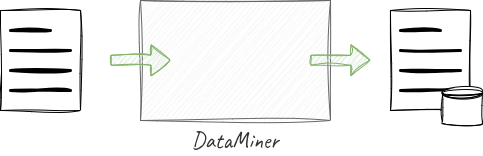
\includegraphics[scale=0.5]{./chapter/images/chapter_1.overview}
        \caption{Esquema general del sistema. \textit{Elaboración propia.}}
        \label{fig:chapter_1.overview}
    \end{center}
\end{figure}

\todo[inline]{@TODO: Mejorar la figura}

Tal y como se puede ver en la figura \ref{fig:chapter_1.overview}
el sistema recibe documentos y genera información en un formato estructurado.
El tipo de estructura, dependerá del tipo de documento.
Por ejemplo en un contrato de alquiler de vivienda aparecerán los datos de la vivienda, y en un contrato de compraventa
de vehículos, aparecerán los datos del vehículo.
